\documentclass[12pt]{article}
\usepackage[english]{babel}
\usepackage[utf8x]{inputenc}
\usepackage[T1]{fontenc}
\usepackage{scribe}
\usepackage{listings}
\usepackage{algorithm}
\usepackage{mathtools}
\usepackage{algorithmicx}
\usepackage{algpseudocode}
\usepackage{fancyhdr}
\usepackage{extramarks}
\usepackage{hyperref}
\usepackage{cleveref}
%\usepackage[style=authoryear]{biblatex}
\renewcommand{\Pr}{{\bf Pr}}
\newcommand{\Prx}{\mathop{\bf Pr\/}}
\newcommand{\E}{{\bf E}}
\newcommand{\Ex}{\mathop{\bf E\/}}
\newcommand{\Var}{{\bf Var}}
\newcommand{\Varx}{\mathop{\bf Var\/}}
\newcommand{\Cov}{{\bf Cov}}
\newcommand{\Cor}{{\bf Corr}}
\newcommand{\Covx}{\mathop{\bf Cov\/}}
\newcommand{\rank}{\text{rank}}

% shortcuts for symbol names that are too long to type
\newcommand{\eps}{\epsilon}
\newcommand{\lam}{\lambda}
\renewcommand{\l}{\ell}
\newcommand{\la}{\langle}
\newcommand{\ra}{\rangle}
%\newcommand{\wh}{\widehat}

% "blackboard-fonted" letters for the reals, naturals etc.
\newcommand{\R}{\mathbb R}
\newcommand{\N}{\mathbb N}
\newcommand{\Z}{\mathbb Z}
\newcommand{\F}{\mathbb F}
\newcommand{\Q}{\mathbb Q}
%\newcommand{\C}{\mathbb C}
\DeclareMathOperator{\Tr}{Tr}

% operators that should be typeset in Roman font
\newcommand{\poly}{\mathrm{poly}}
\newcommand{\polylog}{\mathrm{polylog}}
\newcommand{\sgn}{\mathrm{sgn}}
\newcommand{\avg}{\mathop{\mathrm{avg}}}
\newcommand{\val}{{\mathrm{val}}}

% complexity classes
\renewcommand{\P}{\mathrm{P}}
\newcommand{\NP}{\mathrm{NP}}
\newcommand{\BPP}{\mathrm{BPP}}
\newcommand{\DTIME}{\mathrm{DTIME}}
\newcommand{\ZPTIME}{\mathrm{ZPTIME}}
\newcommand{\BPTIME}{\mathrm{BPTIME}}
\newcommand{\NTIME}{\mathrm{NTIME}}

% values associated to optimization algorithm instances
\newcommand{\Opt}{{\mathsf{Opt}}}
\newcommand{\Alg}{{\mathsf{Alg}}}
\newcommand{\Lp}{{\mathsf{Lp}}}
\newcommand{\Sdp}{{\mathsf{Sdp}}}
\newcommand{\Exp}{{\mathsf{Exp}}}

% if you think the sum and product signs are too big in your math mode; x convention
% as in the probability operators
\newcommand{\littlesum}{{\textstyle \sum}}
\newcommand{\littlesumx}{\mathop{{\textstyle \sum}}}
\newcommand{\littleprod}{{\textstyle \prod}}
\newcommand{\littleprodx}{\mathop{{\textstyle \prod}}}

% horizontal line across the page
\newcommand{\horz}{
\vspace{-.4in}
\begin{center}
\begin{tabular}{p{\textwidth}}\\
\hline
\end{tabular}
\end{center}
}

% calligraphic letters
\newcommand{\calA}{{\cal A}}
\newcommand{\calB}{{\cal B}}
\newcommand{\calC}{{\cal C}}
\newcommand{\calD}{{\cal D}}
\newcommand{\calE}{{\cal E}}
\newcommand{\indep}{\rotatebox[origin=c]{90}{$\models$}}
\newcommand{\calF}{{\cal F}}
\newcommand{\calG}{{\cal G}}
\newcommand{\calH}{{\cal H}}
\newcommand{\calI}{{\cal I}}
\newcommand{\calJ}{{\cal J}}
\newcommand{\calK}{{\cal K}}
\newcommand{\calL}{{\cal L}}
\newcommand{\calM}{{\cal M}}
\newcommand{\calN}{{\cal N}}
\newcommand{\calO}{{\cal O}}
\newcommand{\calP}{{\cal P}}
\newcommand{\calQ}{{\cal Q}}
\newcommand{\calR}{{\cal R}}
\newcommand{\calS}{{\cal S}}
\newcommand{\calT}{{\cal T}}
\newcommand{\calU}{{\cal U}}
\newcommand{\calV}{{\cal V}}
\newcommand{\calW}{{\cal W}}
\newcommand{\calX}{{\cal X}}
\newcommand{\calY}{{\cal Y}}
\newcommand{\calZ}{{\cal Z}}
\newcommand{\com}{^\complement}
\newcommand{\inv}{^{-1}}
\newcommand{\tp}{^\top}
% bold letters (useful for random variables)
\renewcommand{\a}{{\boldsymbol a}}
\renewcommand{\b}{{\boldsymbol b}}
\renewcommand{\c}{{\boldsymbol c}}
\renewcommand{\d}{{\boldsymbol d}}
\newcommand{\e}{{\boldsymbol e}}
\newcommand{\f}{{\boldsymbol f}}
\newcommand{\g}{{\boldsymbol g}}
\newcommand{\h}{{\boldsymbol h}}
\renewcommand{\i}{{\boldsymbol i}}
\renewcommand{\j}{{\boldsymbol j}}
\renewcommand{\k}{{\boldsymbol k}}
\newcommand{\m}{{\boldsymbol m}}
\newcommand{\n}{{\boldsymbol n}}
\renewcommand{\o}{{\boldsymbol o}}
\newcommand{\p}{{\boldsymbol p}}
\newcommand{\q}{{\boldsymbol q}}
\renewcommand{\r}{{\boldsymbol r}}
\newcommand{\s}{{\boldsymbol s}}
\renewcommand{\t}{{\boldsymbol t}}
\renewcommand{\u}{{\boldsymbol u}}
\renewcommand{\v}{{\boldsymbol v}}
\newcommand{\w}{{\boldsymbol w}}
\newcommand{\x}{{\boldsymbol x}}
\newcommand{\y}{{\boldsymbol y}}
\newcommand{\z}{{\boldsymbol z}}
\newcommand{\A}{{\boldsymbol A}}
\newcommand{\B}{{\boldsymbol B}}
\newcommand{\D}{{\boldsymbol D}}
%\newcommand{\G}{{\boldsymbol G}}
\renewcommand{\H}{{\boldsymbol H}}
\newcommand{\I}{{\boldsymbol I}}
\newcommand{\J}{{\boldsymbol J}}
\newcommand{\K}{{\boldsymbol K}}
\renewcommand{\L}{{\boldsymbol L}}
\newcommand{\M}{{\boldsymbol M}}
\renewcommand{\O}{{\boldsymbol O}}
\renewcommand{\S}{{\boldsymbol S}}
\newcommand{\T}{{\boldsymbol T}}
%\newcommand{\U}{{\boldsymbol U}}
\newcommand{\V}{{\boldsymbol V}}
\newcommand{\W}{{\boldsymbol W}}
\newcommand{\X}{{\boldsymbol X}}
\newcommand{\Y}{{\boldsymbol Y}}
\newcommand{\bra}[1]{\left(#1\right)}
\newcommand{\bgbra}[1]{\left\{#1\right\}}
\newcommand{\abs}[1]{\left|#1\right|}
\newcommand{\innprod}[1]{\left\langle#1\right\rangle}
\newcommand{\norm}[1]{\left\|#1\right\|}
\newcommand{\wh}[1]{\widehat{#1}}
\newcommand{\wt}[1]{\widetilde{#1}}
\newcommand{\srt}{^{\frac{1}{2}}}
\newcommand{\idx}[1]{^{\bra{#1}}}
\def\beq{\begin{equation}}
\def\eeq{\end{equation}}
\def\bal{\begin{aligned}}
\def\eal{\end{aligned}}
\def\beqal{\begin{equation}\begin{aligned}}
\def\eeqal{\end{aligned}\end{equation}}
\def\nbeqal{\[ \bal}
\def\neeqal{\eal \]}
\newcommand{\mtline}[1]{\beq
\left\{
\bal
#1
\eal
\right.
\eeq}


% useful for Fourier analysis
\newcommand{\bits}{\{-1,1\}}
\newcommand{\bitsn}{\{-1,1\}^n}
\newcommand{\bn}{\bitsn}
\newcommand{\isafunc}{{: \bitsn \rightarrow \bits}}
\newcommand{\fisafunc}{{f : \bitsn \rightarrow \bits}}
\newcommand{\ndone}{\frac{1}{n}}
\newcommand{\supp}{\text{supp}}
\newcommand*\Let[2]{\State #1 $\gets$ #2}


\makeatletter
\newcommand{\distas}[1]{\mathbin{\overset{#1}{\kern\z@\sim}}}%
\newsavebox{\mybox}\newsavebox{\mysim}
\newcommand{\distras}[1]{%
  \savebox{\mybox}{\hbox{\kern3pt$\scriptstyle#1$\kern3pt}}%
  \savebox{\mysim}{\hbox{$\sim$}}%
  \mathbin{\overset{#1}{\kern\z@\resizebox{\wd\mybox}{\ht\mysim}{$\sim$}}}%
}
\makeatother
\newcommand{\iid}{\distras{\text{i.i.d.}}}
\makeatletter
\newcommand*{\rom}[1]{\expandafter\@slowromancap\romannumeral #1@}
\makeatother

% if you want
\newcommand{\half}{{\textstyle \frac12}}

\newcommand{\myfig}[4]{\begin{figure}[h] \begin{center} \includegraphics[width=#1\textwidth]{#2} \caption{#3} \label{#4} \end{center} \end{figure}} 
\newcommand{\chara}{\mathbb{1}}

\Scribe{Xinze Li}
\Lecturer{Chao Gao}
\LectureNumber{12}
\LectureDate{Feb 17, 2020}
\LectureTitle{Isotonic Regression}

\lstset{style=mystyle}



\begin{document}
	\MakeScribeTop
\section{Problem Formulation}
Isotonic regression is also called shape-constraint estimation. The advantage of this kind of estimation is that we do not need tuning parameter to do the estimation. We assume the nonparametric model as follows
\[
y_i=f(x_i)+z_i,\quad i\in[n],z_i\iid \calN(0,\sigma^2)
\]
We also assume that $f$ is nondecreasing. In particular, we suppose
\beq\bal
y_i=\theta_i+z_i,\quad z_i&\iid\calN(0,\sigma^2),\quad i\in[n]\\
\theta_1\leq\theta_2\leq&\cdots\leq \theta_n
\eal\eeq
So we could compute the following estimator
\beq\label{probcvx}
\wh{\theta}=\arg\min_{\theta_1\leq\theta_2\leq\cdots\leq \theta_n}\norm{y-\theta}^2
\eeq
Note that the constraint is linear, and the objective is quadratic, so this is an easy quadratic programmming problem. In particular, this is a convex programming problem, which is easily computable. We define the following convex set naturally
\beq
C=\bgbra{\theta\in\R^n:\theta_1\leq\theta_2\leq \cdots\leq \theta_n}
\eeq
We also construct the vector $v_j=\sum_{i=1}^j e_j$, where $\{e_j\}_{j=1}^n$ is the canonical base of $\R^n$. Now note that $\wh{\theta}\in C$, and that for every $\eps>0$, $\wh{\theta}-\eps v_j\in C$, so we could derive the basic inequality.
\beq
\norm{\wh{\theta}-y}^2\leq \norm{\wh{\theta}-\eps v_j-y}^2
\eeq
Expanding the RHS gives
\[
0\leq \eps j-2\innprod{\wh{\theta}-y, v_j}
\]
Let $\eps$ goes to zero gives
\[
\innprod{\wh{\theta}-y, v}\leq 0
\]
In other words,
\beq
\sum_{i=1}^j \wh{\theta}_i\leq \sum_{i=1}^j y_i, \quad \forall j\in[n]
\eeq
Now notice that if $\wh{\theta}_j<\wh{\theta}_{j+1}$, the inequality strictly holds, then for $\eps$ sufficiently small, we have $\wh{\theta}+\eps v_j\in C$. Following the same computation gives
\[
\innprod{\wh{\theta}-y, v_j}\geq 0
\]
Combining these reasoning, we have the following characterization of $\wh{\theta}$
\mtline{
&\sum_{i=1}^j\wh{\theta}_i\leq \sum_{i=1}^j y_i\quad \forall j\in [n]\\
&\sum_{i=1}^j\wh{\theta}_i= \sum_{i=1}^j y_i\quad \forall j\text{ s.t. }\wh{\theta}_j<\wh{\theta}_{j+1}\text{ or }j=n\\
}
We could also observe that the solution is unique (because the objective is strongly convex) and that the curve of the sum of $\theta_i$ is the largest convex function below the curve of the sum of $y_i$ (including $(0,0)$). 
\begin{figure}[htbp]
  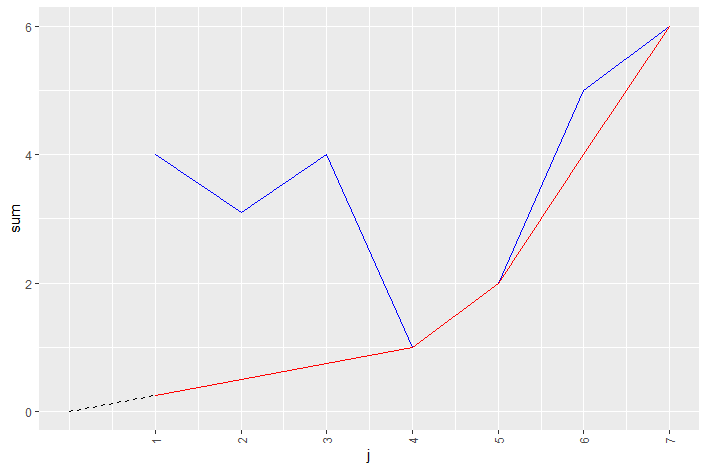
\includegraphics[width=\linewidth]{plt1.png}
  \caption{Simple Example of Convex Minorant}
  \label{fig:boat1}
\end{figure}
Let $f$ be an arbitrary continuous function, then we could define $\bar{f}$ as the convex minorant of $f$, i.e., the largest convex function that is smaller than or equal to $f$ everywhere. We could also define the right derivative of $\bar{f}$ as
\nbeqal
\bar{f}^{(1,r)}(t)&=\inf_{w>t}\sup_{s\leq t}\frac{f(w)-f(s)}{w-s}\\
&=\sup_{s\leq t}\inf_{w>t}\frac{f(w)-f(s)}{w-s}\\
\neeqal
We could also define the left derivative similarly. We now could conclude that the solution to the convex programming problem~\ref{probcvx} is
\beq
\wh{\theta_i}=\min_{l\geq i}\max_{k\leq i}\bar{y}_{[k,l]},\quad \bar{y}_{[k,l]}=\frac{1}{l-k+1}\sum_{j=k}^l y_j
\eeq
We could use \textbf{PAVA} (pool-adjacent-violators-algorithm) to get the solution in linear time.
\section{Algorithm}
PAVA algorithm is easy to describe. It works just as its name says: to pool adjacent violators. So we first scan the array from the first element to the last element. Once there is a violator $y_i>y_{i+1}$, we pool these two nodes together to be a single node, with weight $2$ and value equal to the weighted average. Because once we do these pooling procedure, the length of the array decrease by one, the time complexity of the algorithm is $O(n)$. We now verify the correctness of the algorithm. \\
First note that if $y_1\leq y_2\leq\cdots\leq y_n$ already, then
\[
y=\arg\min_{\theta\leq\cdots\leq \theta_n}\sum_{i=1}^n w_i\bra{y_i-\theta_i}^2
\]
Suppose $y_5>y_6$ for simplicity. It is easy to note that
\[
\min_{\theta_1\leq\cdots\leq\theta_n}\sum_{i=1}^n w_i\bra{y_i-\theta_i}^2=\min_{\theta_1\leq\cdots\leq \theta_5=\theta_6\leq\cdots\leq\theta_n}\sum_{i=1}^n w_i\bra{y_i-\theta_i}^2
\]
This is because if $\theta_5<\theta_6$ strictly, then we could always pull $\theta_5$ towards $\theta_6$ or pull $\theta_6$ towards $\theta_5$, to decrease the objective value, and in the same time still maintain the isotonic property. We could then write
\[\bal
w_5\bra{y_5-\theta}^2+w_6\bra{y_6-\theta}^2&=\bra{w_5+w_6}\bra{\frac{w_5y_5+w_6y_6}{w_5+w_6}-\theta}^2+w_5\bra{y_5-\frac{w_5y_5+w_6y_6}{w_5+w_6}}^2\\&+w_6\bra{y_6-\frac{w_5y_5+w_6y_6}{w_5+w+6}}^2
\\&=\bra{w_5+w_6}\bra{\frac{w_5y_5+w_6y_6}{w_5+w_6}-\theta}^2+f(y_5,y_6,w_5,w_6)
\eal\]
Thus, we have
\[\bal
\arg\min_{\theta\leq\cdots\leq \theta_n}\sum_{i=1}^n w_i\bra{y_i-\theta_i}^2&=\arg\min_{\theta_1\leq\cdots\leq \theta_4\leq\theta\leq\theta_7\leq\cdots\leq \theta_n} \left[\sum_{i=1}^4w_i\bra{y_i-\theta_i}^2\right.\\&+ \left.\bra{w_5+w_6}\bra{\frac{w_5y_5+w_6y_6}{w_5+w_6}-\theta}^2 +\sum_{i=7}^n w_i\bra{y_i-\theta_i}^2 \right]
\eal\]
And this is exactly what the algorithm is doing.
\section{Property of PAVA Estimator}
\begin{theorem}[Meyer-Woodroofe-Zhang]
If $\theta_n-\theta_1\leq V$, then 
\beq
\E \norm{\wh{\theta}-\theta}^2\lesssim \sigma^2\bra{\log (en) + n^{1/3}\bra{\frac{V}{\sigma}}^{2/3} }
\eeq
\end{theorem}
\begin{remark}
Suppose $\theta$ is a piecewise constant function with $K$ blocks and that if $\theta_i\in j_{th}$ block, then $\theta_i=\mu_j$. Now note that if we let $\wh{\theta}_i$ be the average value of all $y_i$ in the $j_th$ block, then we have
\[
\E\norm{\wh{\theta}-\theta}^2=\sum_{i=1}^n\bra{\wh{\theta}_i-\theta_i}^2=\sum_{j=1}^{K}\bra{\sum_{i\in B_j} \frac{\sigma^2}{n_j}}=\sigma^2K
\]
where $B_j$ is the set of all elements in the $j_{th}$ block. Another case is when $\frac{V}{\sigma}=O(1)$, then $E\norm{\wh{\theta}-\theta}^2\preceq \sigma^2 n^{1/3}$. This indicates that $n$ elements are divided into $O(n^{1/3})$ pieces.
\end{remark}
\begin{proof}
Following the above notation, and let
\beq
\wh{\theta}_i=\min_{l\geq i}\max_{k\leq i} \bar{y}_{[k,l]}
\eeq
Also use the following notation
\[
x_+=\max(0, x),\quad x_-=\max(0, -x),\quad \abs{x}=x_++x_-
\]
Then we have
\[
\E\norm{\wh{\theta}-\theta}^2=\sum_{i=1}^n\E\norm{\wh{\theta}-\theta}_+^2+\E\norm{\wh{\theta}-\theta}_-^2
\]
Also
\[
\wh{\theta}_i=\min_{l\geq i}\max_{k\leq i} \bar{y}_{[k,l]}\leq \min_{i\leq l\leq i+m_i}\max_{k\leq i} \bra{\bar{\theta}_{[k,l]}+\bar{z}_{[k,l]}}
\]
where $m_i$ is defined as follows
\[
m_i=\max_m\bgbra{m:\bar{\theta}_{[i,i+m]}-\theta_i\leq v(m),i+m\leq n}
\]
$v(m)$ is a bias function to be determined. Using this definition, we have the inequality
\[
\bar{\theta}_{[k,l]}\leq \bar{\theta}_{[i,l]}\leq \theta_i+v(m_i)
\]
Thus,
\[
\wh{\theta}_i\leq \theta_i+v(m_i)+\min_{i\leq l\leq i+m_i}\max_{k\leq i}\bar{z}_{[k,l]}
\]
Rearranging the order gives
\[
\bra{\wh{\theta}_i-\theta_i}_+\leq \bra{v(m_i)+\min_{i\leq l\leq i+m_i}\max_{k\leq i}\bra{z}_{[k,l]}}_+\leq v(m_i)+\bra{\min_{i\leq l\leq i+m_i}\max_{k\leq i}\bra{z}_{[k,l]}}_+
\]
So we have
\beqal
\sum_{i=1}^n\E\bra{\wh{\theta}_i-\theta_i}_+^2&\leq 2\sum_{i=1}^n v(m_i)^2+2\sum_{i=1}^n \E\bra{\min_{i\leq l\leq i+m_i}\max_{k\leq i} \bar{z}_{[k,l]} }_+^2\\
\sum_{i=1}^n\E\bra{\wh{\theta}_i-\theta_i}_-^2&\leq 2\sum_{i=1}^n \E\bra{\min_{i\leq l\leq i+m_i}\max_{k\leq i} \bar{z}_{[k,l]} }_-^2\\
\eeqal
Combining these two inequalities gives
\[
\E\norm{\wh{\theta}-\theta}^2\leq 2\sum_{i=1}^n v(m_i)^2+2\sum_{i=1}^n \E\bra{\min_{i\leq l\leq i+m_i}\max_{k\leq i} \bar{z}_{[k,l]} }^2
\]
Before we do the next analysis, we first recall knowledge in probability theory. We say that $\bra{\calF_i}_{i=1}^\infty$ is a filtration if $\calF_1\subseteq\calF_2\subseteq\cdots$. And that $\bra{X_t}$ is a (sub)martingale if the following two requirements are met:
\begin{enumerate}
\item $X_t$ is an adaptive process, i.e., it is measurable w.r.t. $\calF_t$.
\item $\E\bra{X_t|\calF_{t-1}} (\geq)=X_{t-1} $.
\end{enumerate}
An obvious but interesting fact is that if $\phi$ is a convex function and $\bra{X_t}$ is a martingale w.r.t. $\calF_t$, then $\bra{\phi(X_t)}$ is a submartingale. This is just a one-line proof:
\[
\E\bra{\phi\bra{X_t}|\calF_{t-1}}\geq \phi\bra{\E\bra{X_t|\calF_{t-1}}}=\phi\bra{X_{t-1}}
\]
We now introduce Doob's maximal inequality
\begin{lemma}
If $\bra{M_n}_{n=1}^\infty$ is a positive submartingale, then
\[
\E\bra{\max_{1\leq m\leq n}M_m}^2\leq 4\E M_n^2
\]
\end{lemma}
\begin{example}
Suppose $z_i\iid P$, and have finite second moment: $\E z_i^2<\infty$. Let $S_n$ be the mean of the first $n$ elements: $S_n=\frac{1}{n}\sum_{i=1}^n z_i$. Then we claim that $S_n$ is a reverse martingale
\[
\E\bra{S_{n-1}|S_n}=\frac{1}{n-1}\sum_{i=1}^{n-1}\E\bra{z_i|S_n}=\frac{1}{n-1}S_n=S_n
\]
The second equality holds because the best guess of $z_i$ when we know $S_n$ is just $S_n$.
\end{example}
Using this, we could prove that
\[
\bal
\E\bra{\min_{i\leq l\leq i+m_i}\max_{k\leq i} \bar{z}_{[k,l]}}_+^2&\leq \E \bra{\max_{k\leq i}\bar{z}_{[k,i+m_i]}}_+^2\\
&\leq 4 \E\bra{\bar{z}_{[i,i+m_i]}}_+^2\\
&=\frac{4}{m_i+1}\E \bra{\calN(0,\sigma^2)}_+^2\\
&\lesssim \frac{\sigma^2}{m_i+1}
\eal
\]
So we could write
\[
\E\norm{\wh{\theta}-\theta}^2\lesssim\sum_{i=1}^n \bra{v(m_i)+\frac{\sigma^2}{m_i+1}}
\]
To balance variance and bias, we choose \[
v(m)^2=\frac{\sigma^2}{m+1}
\]
So we have the following analysis
\nbeqal
\E\norm{\wh{\theta}-\theta}^2&\lesssim \sigma^2\sum_{i=1}^n \frac{1}{m_i+1}\\
&=\sigma^2\sum_{i=1}^n\sum_{l\geq 0}\chara\bra{2^l\leq m_i< 2^{l+1}}\frac{1}{m_i+1}+\sigma^2\sum_{i=1}^n \chara\bra{0\leq m_i< 1}\frac{1}{m_i+1}\\
&\leq \sigma^2\sum_{l\geq 0}\frac{1}{2^l+1}\sum_{i=1}^n \chara\bra{2^l\leq m_i<2^{l+1}}+\sigma^2\sum_{i=1}^n \chara\bra{0\leq m_i<1}\\
&=\sigma^2\sum_{l\geq 0}\frac{1}{2^l+1}\bra{H\bra{2^{l+1}}-H\bra{2^l} }+\sigma^2H(1)
\neeqal
where
\[
H(m)=\sum_{i=1}^n\chara\bra{m_i\leq m}
\]
So if $H(m)\leq \wt{H}(m)$ for every $m\geq 0$, then
\[
\sigma^2\sum_{l\geq 0}\frac{1}{2^l+1}\bra{H\bra{2^{l+1}}-H\bra{2^l} }+\sigma^2H(1)\leq \sigma^2\sum_{l\geq 0}\frac{1}{2^l+1}\bra{\wt{H}\bra{2^{l+1}}-\wt{H}\bra{2^l} }+\sigma^2\wt{H}(1)
\]
Now recall $m_i$'s defintion
\[
m_i=\max_m\bgbra{m:\bar{\theta}_{[i,i+m]}-\theta_i\leq v(m),i+m\leq n}
\]
thus if $m_i<m$, then $\bar{\theta}_{[i,i+m]}>v(m)$. Thus, we have
\[\bal
H(m)&=\sum_{i=1}^n\chara\bra{m_i\leq m}\\&\leq\sum_{i=1}^{n-m}\chara\bra{\bar{\theta}_{[i, i+m]}-\theta_i>v(m) } +m\\
&\leq \sum_{i=1}^{n-m}\frac{\bar{\theta}_{[i, i+m]}-\theta_i}{v(m)}+m\\
&\leq \sum_{i=1}^{n-m} \frac{\theta_{i+m}-\theta_i}{v(m)}+m\\
&\leq \frac{mV}{v(m)}+m\\
&=m+\frac{mV}{\sigma}\sqrt{m+1}
\eal\]
The last inequality holds because all terms are canceled except for the first $m$ and the last $m$ term and they form $m$ pairs. Then the bound is derived because of the total variation is $V$. So we have a bound for $H(m)$:
\[
H(m)\leq \min\bra{n, m\sqrt{m+1}\cdot \frac{V}{\sigma}}+\min\bra{n,m}=\wt{H}(m)
\]
So now we have the analysis
\[\bal
\E\norm{\wh{\theta}-\theta}^2&\lesssim \sigma^2\cdot \sum_{l\geq 0}\frac{1}{2^l+1}\bra{\wt{H}\bra{2^{l+1}}-\wt{H}\bra{2^l} }+\sigma^2\wt{H}(1)\\
&=\sigma^2\cdot\underbrace{\sum_{l\geq 0}\frac{1}{2^l+1}\left[ \min\bra{n, 2^{l+1}\sqrt{2^{l+1}+1}\cdot \frac{V}{\sigma}}-\min\bra{n, 2^{l}\sqrt{2^{l}+1}\cdot \frac{V}{\sigma}} \right]}_{\text{\rom{1}}}\\
&+\sigma^2\cdot \underbrace{\sum_{l\geq 0} \frac{1}{2^l+1}\left[\min\bra{n,2^{l+1}} -\min\bra{n,2^l} \right]}_{\text{\rom{2}}}+\sigma^2\cdot\underbrace{\bra{\min\bra{n,\frac{V}{\sigma}}+1}}_{\text{\rom{3}}}
\eal\]
For the second part \rom{2}
\[
\text{\rom{2}}\leq \sum_{2^l\leq n}\frac{1}{2^l+1}\min\bra{n,2^{l+1}}\leq \sum_{2^l\leq n}2\lesssim \log\bra{en}
\]
And the first part \rom{1} is just the same analysis
\[\bal
\text{\rom{1}}&\leq \sum_{2^l\sqrt{2^l+1}V/\sigma\leq n}\frac{1}{2^l+1}\min\bra{n, 2^{l+1}\sqrt{2^{l+1}+1 }\cdot \frac{V}{\sigma} }\\
&\lesssim \sum_{2^{3l/2}\leq n\sigma/V}2^\frac{l}{2}\frac{V}{\sigma}\\
&\lesssim \bra{n\frac{\sigma}{V}}^{\frac{2}{3}\times\frac{1}{2}}\cdot \frac{V}{\sigma}\\
&= n^\frac{1}{3}\cdot \bra{\frac{V}{\sigma}}^\frac{2}{3}
\eal\]
And the third part \rom{3}
\[
\text{\rom{3}}\lesssim n^\frac{1}{3}\cdot \bra{\frac{V}{\sigma}}^\frac{2}{3}
\]
Thus, we conclude that
\[
\E \norm{\wh{\theta}-\theta}^2\lesssim \sigma^2\bra{\log (en) + n^{1/3}\bra{\frac{V}{\sigma}}^{2/3} }
\]
\end{proof}
Actually, we could prove that
\begin{theorem}[\cite{zhang2002}]
\beq\sum_{i=n_1}^{n_2}\E\bra{\wh{\theta}_i-\theta_i}^2\lesssim \sigma^2\left[\log\bra{e(n_2-n_1)} +\bra{n_2-n_1}^\frac{1}{3}\cdot \bra{\frac{\theta_{n_2}-\theta_{n_1}}{\sigma}^\frac{2}{3}} \right]\eeq
\end{theorem}
For more details, see homework 9.
If we assume that \begin{equation}\begin{aligned}
&\Theta_{k}^{\uparrow}=\left\{\theta \in \mathbb{R}^{n}: \text { there exist }\left\{a_{j}\right\}_{j=0}^{k} \text { and }\left\{\mu_{j}\right\}_{j=1}^{k}\text { such that }\right.\\
&\begin{array}{l}
0=a_{0} \leq a_{1} \leq \cdots \leq a_{k}=n \\
\left.\mu_{1} \leq \mu_{2} \leq \cdots \leq \mu_{k}, \text { and } \theta_{i}=\mu_{j} \text { for all } i \in\left(a_{j-1}: a_{j}\right]\right\}
\end{array}
\end{aligned}\end{equation}
the parameter space of nondecreasing vectors with at most $k$ pieces. Then we have that if $\theta\in\Theta_{k}^\uparrow$, then 
\[
\E \norm{\wh{\theta}-\theta}^2\lesssim \sigma^2\sum_{j=1}^{k}\log\bra{en_j}
\]
where $n_j$ is the length of each pieces. Combining these two results, we know that if $\theta$ has at most $k$ pieces, monotone and have total variation at most $V$, then
\[
\E \norm{\wh{\theta}-\theta}^2\lesssim \sigma^2\min\bgbra{\log\bra{en}+n^{1/3}\bra{\frac{V}{\sigma}}^{2/3}, k\log\bra{\frac{en}{k}} }
\]
And from~\cite{gao2017estimation}, we know the minimax rate
\begin{equation}\inf _{\widehat{\theta}} \sup _{\theta^{*} \in \Theta_{k}^{\uparrow}} \mathbb{E}\left\|\widehat{\theta}-\theta^{*}\right\|^{2} \geq\left\{\begin{array}{ll}
c \sigma^{2}, & k=1 \\
c \sigma^{2} k \log \log (16 n / k), & k \geq 2
\end{array}\right.\end{equation}
We could achieve the minimax rate using the following estimator
\[
\wh{\theta}=\arg\min_{\theta\in\Theta_{k}^\uparrow}\norm{y-\theta}^2
\] 
The $\log\log$ term appears because of the law of iterated logarithm
\[
\max_{1\leq m\leq n}\abs{\frac{1}{\sqrt{m}}\sum_{i=1}^m z_i}\asymp\sigma\sqrt{\log\log n},\quad z_i\iid \calN(0, \sigma^2)
\]
Also if we define
\[
\Theta^\uparrow(V)=\bgbra{\theta\in\R^n,\theta_1\leq\cdots\leq \theta_n,\theta_n-\theta_1\leq V}
\]
then we have
\[
\inf_{\wh{\theta}}\sup_{\theta \in \Theta^{\uparrow}}\E\norm{\wh{\theta}-\theta}^2\asymp \sigma^2n^{1/3}\bra{\frac{V}{\sigma}}^{2/3}
\]
This is a result from Polyak, Nemirovski and Tsybakov.
























\bibliographystyle{apalike}
\bibliography{IsotonicRegression.bib}	
%%%%%%%%%%% end of doc
\end{document}